\section{V2V-PoseNet}
\label{V2V-PoseNet_Section}

\subsection{Building block design}
We use four kinds of building blocks in designing the V2V-PoseNet. The first one is the \emph{volumetric basic block} that consists of a volumetric convolution, volumetric batch normalization~\cite{ioffe2015batch}, and the activation function (i.e., ReLU). This block is located in the first and last parts of the network. The second one is the \emph{volumetric residual block} extended from the 2D residual block of option B in ~\cite{he2016deep}. The third one is the \emph{volumetric downsampling block} that is identical to a volumetric max pooling layer. The last one is the \emph{volumetric upsampling block}, which consists of a volumetric deconvolution layer, volumetric batch normalization layer, and the activation function (i.e., ReLU). Adding the batch normalization layer and the activation function to the deconvolution layer helps to ease the learning procedure. The kernel size of the residual blocks is 3$\times$3$\times$3 and that of the downsampling and upsampling layers is 2$\times$2$\times$2 with stride 2.


\begin{figure}[t]
\begin{center}
   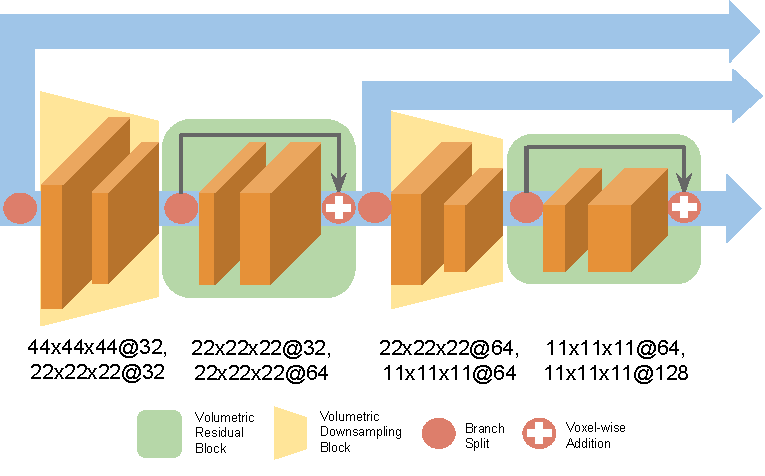
\includegraphics[width=1.0\linewidth]{encoder.pdf}
\end{center}
\vspace*{-5mm}
   \caption{Encoder of the V2V-PoseNet. The numbers below each block indicate the spatial size and number of channels of each feature map. We plotted each feature map without Z-axis to simplify the figure.}
\vspace*{-4mm}
\label{fig:encoder}
\end{figure}


\subsection{Network design}
The V2V-PoseNet performs voxel-to-voxel prediction. Thus, it is based on the 3D CNN architecture that treats the Z-axis as an additional spatial axis so that the kernel shape is $w$$\times$$h$$\times$$d$. Our network architecture is based on the hourglass model~\cite{newell2016stacked}, which was slightly modified for more accurate estimation. As the Figure~\ref{fig:model_architecture} shows, the network starts from the 7$\times$7$\times$7 volumetric basic block and the volumetric downsampling block. After downsampling the feature map, three consecutive residual blocks extract useful local features. The output of the residual blocks goes through the encoder and decoder described in Figures~\ref{fig:encoder} and ~\ref{fig:decoder}, respectively.

In the encoder, the volumetric downsampling block reduces the spatial size of the feature map while the volumetric residual bock increases the number of channels. It is empirically confirmed that this increase in the number of channels helps improve the performance in our experiments. On the other hand, in the decoder, the volumetric upsampling block enlarges the spatial size of the feature map. When upsampling, the network decreases the number of channels to compress the extracted features. The enlargement of the volumetric size in the decoder helps the network to densely localize keypoints because it reduces the stride between voxels in the feature map. The encoder and decoder are connected with the voxel-wise addition for each scale so that the decoder can upsample the feature map more stably. After passing the input through the encoder and decoder, the network predicts the per-voxel likelihood for each keypoint through two 1$\times$1$\times$1 volumetric basic blocks and one 1$\times$1$\times$1 volumetric convolutional layer.


\begin{figure}[t]
\begin{center}
   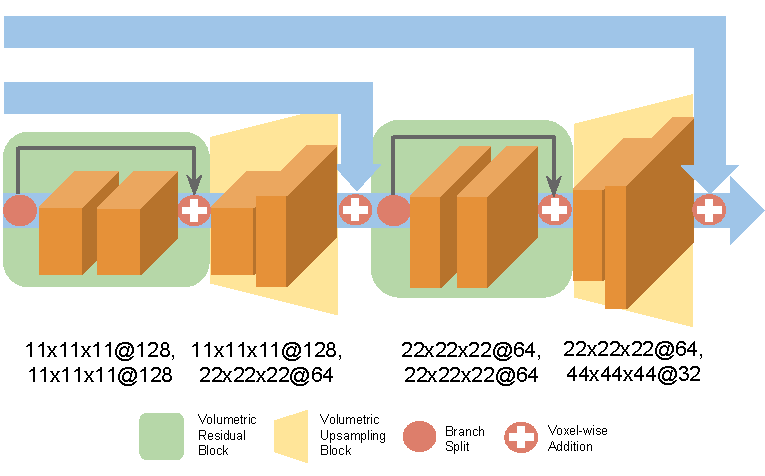
\includegraphics[width=1.0\linewidth]{decoder.pdf}
\end{center}
\vspace*{-5mm}
   \caption{Decoder of the V2V-PoseNet. The numbers below each block indicate the spatial size and number of channels of each feature map. We plotted feature map without Z-axis to simplify the figure.}
\vspace*{-4mm}
\label{fig:decoder}
\end{figure}



\subsection{Network training}
To supervise the per-voxel likelihood for each keypoint, we generate 3D heatmap, wherein the mean of Gaussian peak is positioned at the ground-truth joint location as follows: 

\begin{equation}
H_{\mathrm{n}}^*(i,j,k) = \exp\left(-\frac{(i-i_{\mathrm{n}})^2+(j-j_{\mathrm{n}})^2+(k-k_{\mathrm{n}})^2}{2\sigma^2}\right),
\end{equation}
where $H_{n}^{*}$ is the ground-truth 3D heatmap of $n$th keypoint, ($i_n$,$j_n$,$k_n$) is the ground-truth voxel coordinate of $n$th keypoint, and $\sigma$ = 1.7 is the standard deviation of the Gaussian peak.

Also, we adopt the mean square error as a loss function $L$ as follows:

\begin{equation}
L = \sum_{n=1}^{N} \sum_{i,j,k} \|H_{\mathrm{n}}^*(i,j,k)-H_{\mathrm{n}}(i,j,k)\|^2,
\end{equation}
where $H_{n}^{*}$ and $H_{n}$ are the ground-truth and estimated heatmaps for $n$th keypoint, respectively, and $N$ denotes the number of keypoints.



